\begin{center}
    \textbf{Esta parte corresponde a la parte 'ii.' de esta sección.}
\end{center}

\vspace{.3cm}

Nos dan el siguiente modelo entidad-relación:\\

\begin{center}
    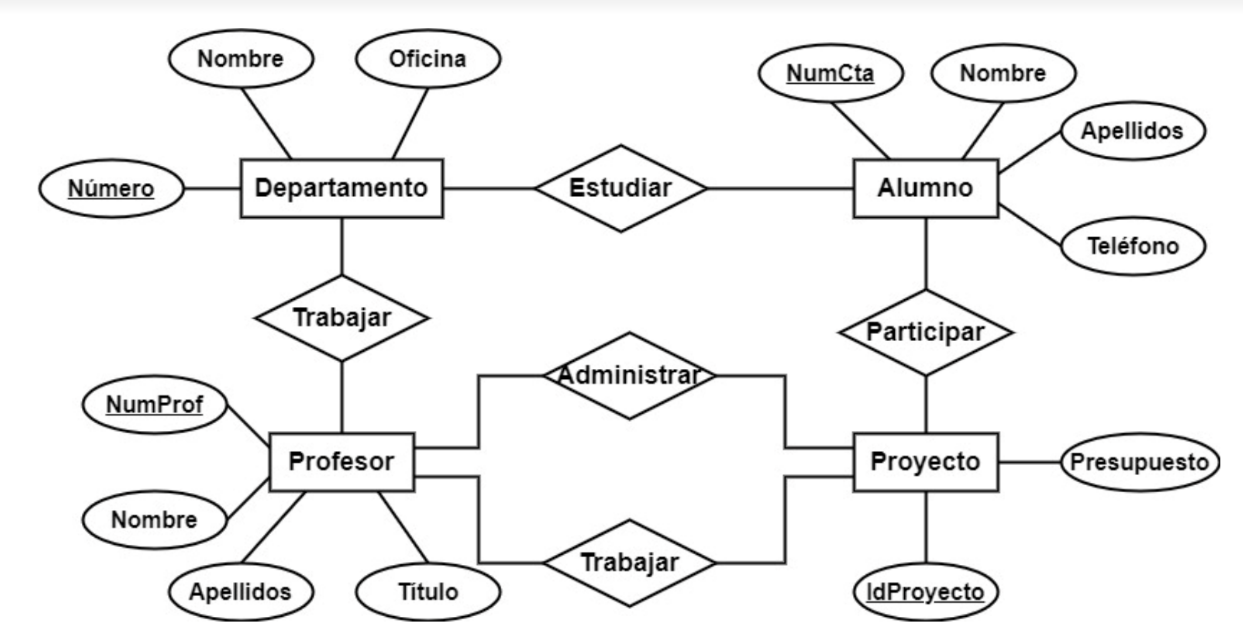
\includegraphics[width=8cm]{resources/ER_2.2.5.png}
\end{center}

Se nos pide obtener un nuevo modelo E-R modificando el anterior bajo ciertas nuevas
especificaciones, hay ciertas restricciones que tuve que interpretar un poco para 
poder traducir, pero aquí está mi interpretación de las mismas:\\
\begin{center}
    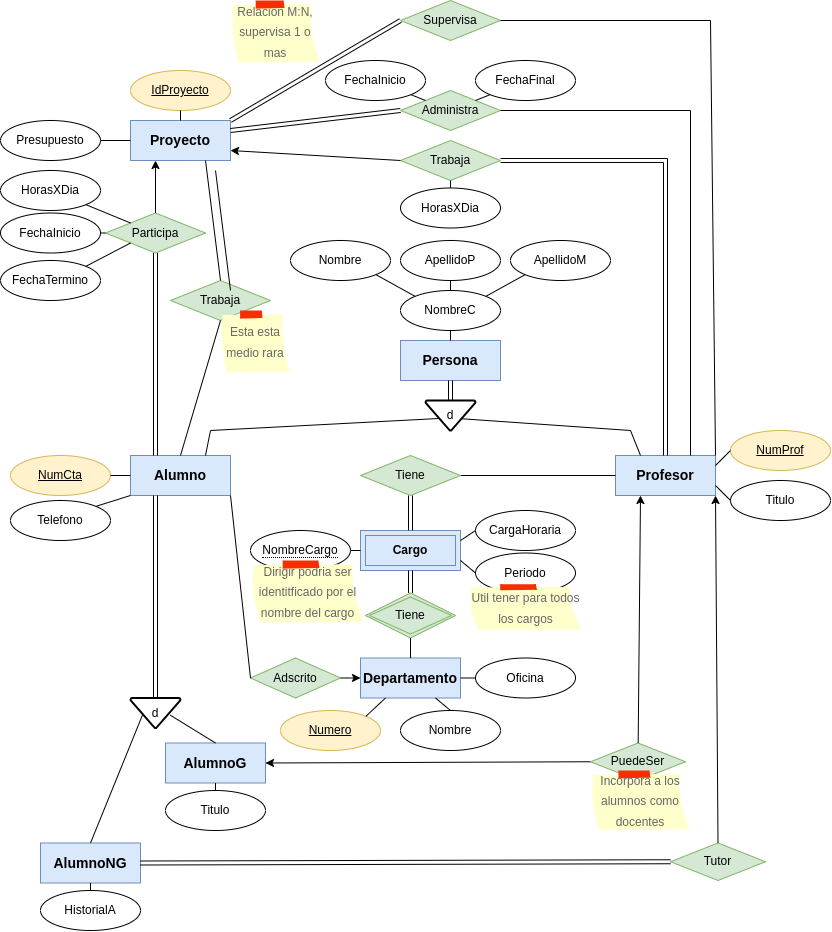
\includegraphics[width=14cm]{resources/Ejercicio_2.5.png}
\end{center}

Incluí algunos comentarios en amarillo sobre cosas que tuve que interpretar un poco,
ademas, agregue color coding para entender mejor las relaciones entre las entidades;
hay una relacion de alumno trabaja en proyecto que veo medio redundante pero bueno.\\